	\documentclass{astroedu-lab}

\begin{document}

\pagestyle{plain}

\begin{problem}{\huge Лабораторная работа 4.3.1\\\\Изучение дифракции света\\\\Выполнил Жданов Елисей Б01-205}

\section{Цель работы:}

1) Исследовать явления дифракции Френеля и Фраунгофера на щели

2) Изучить влияние дифракции на разрешающую способность оптических инструментов

\section{Оборудование:}

Оптическая скамья

Ртутная лампа  

Монохроматор

Щели с регулируемой шириной

Рамка с вертикальной нитью

Двойная щель

Микроскоп на поперечных салазках с микрометрическим винтом

Зрительная труба

\section{Теоретическая справка}

\subsection{Дифракция Френеля на щели}

Схема установки для наблюдения дифракции Френеля на щели представлена на рис. \ref{labA}. Световые лучи освещают щель $ S_2 $ и испытывают на ней дифракцию. Дифракционная картина рассматривается с помощью микроскопа М, сфокусированного на некоторую плоскость наблюдения П.

\begin{figure}[H]
	\centering
	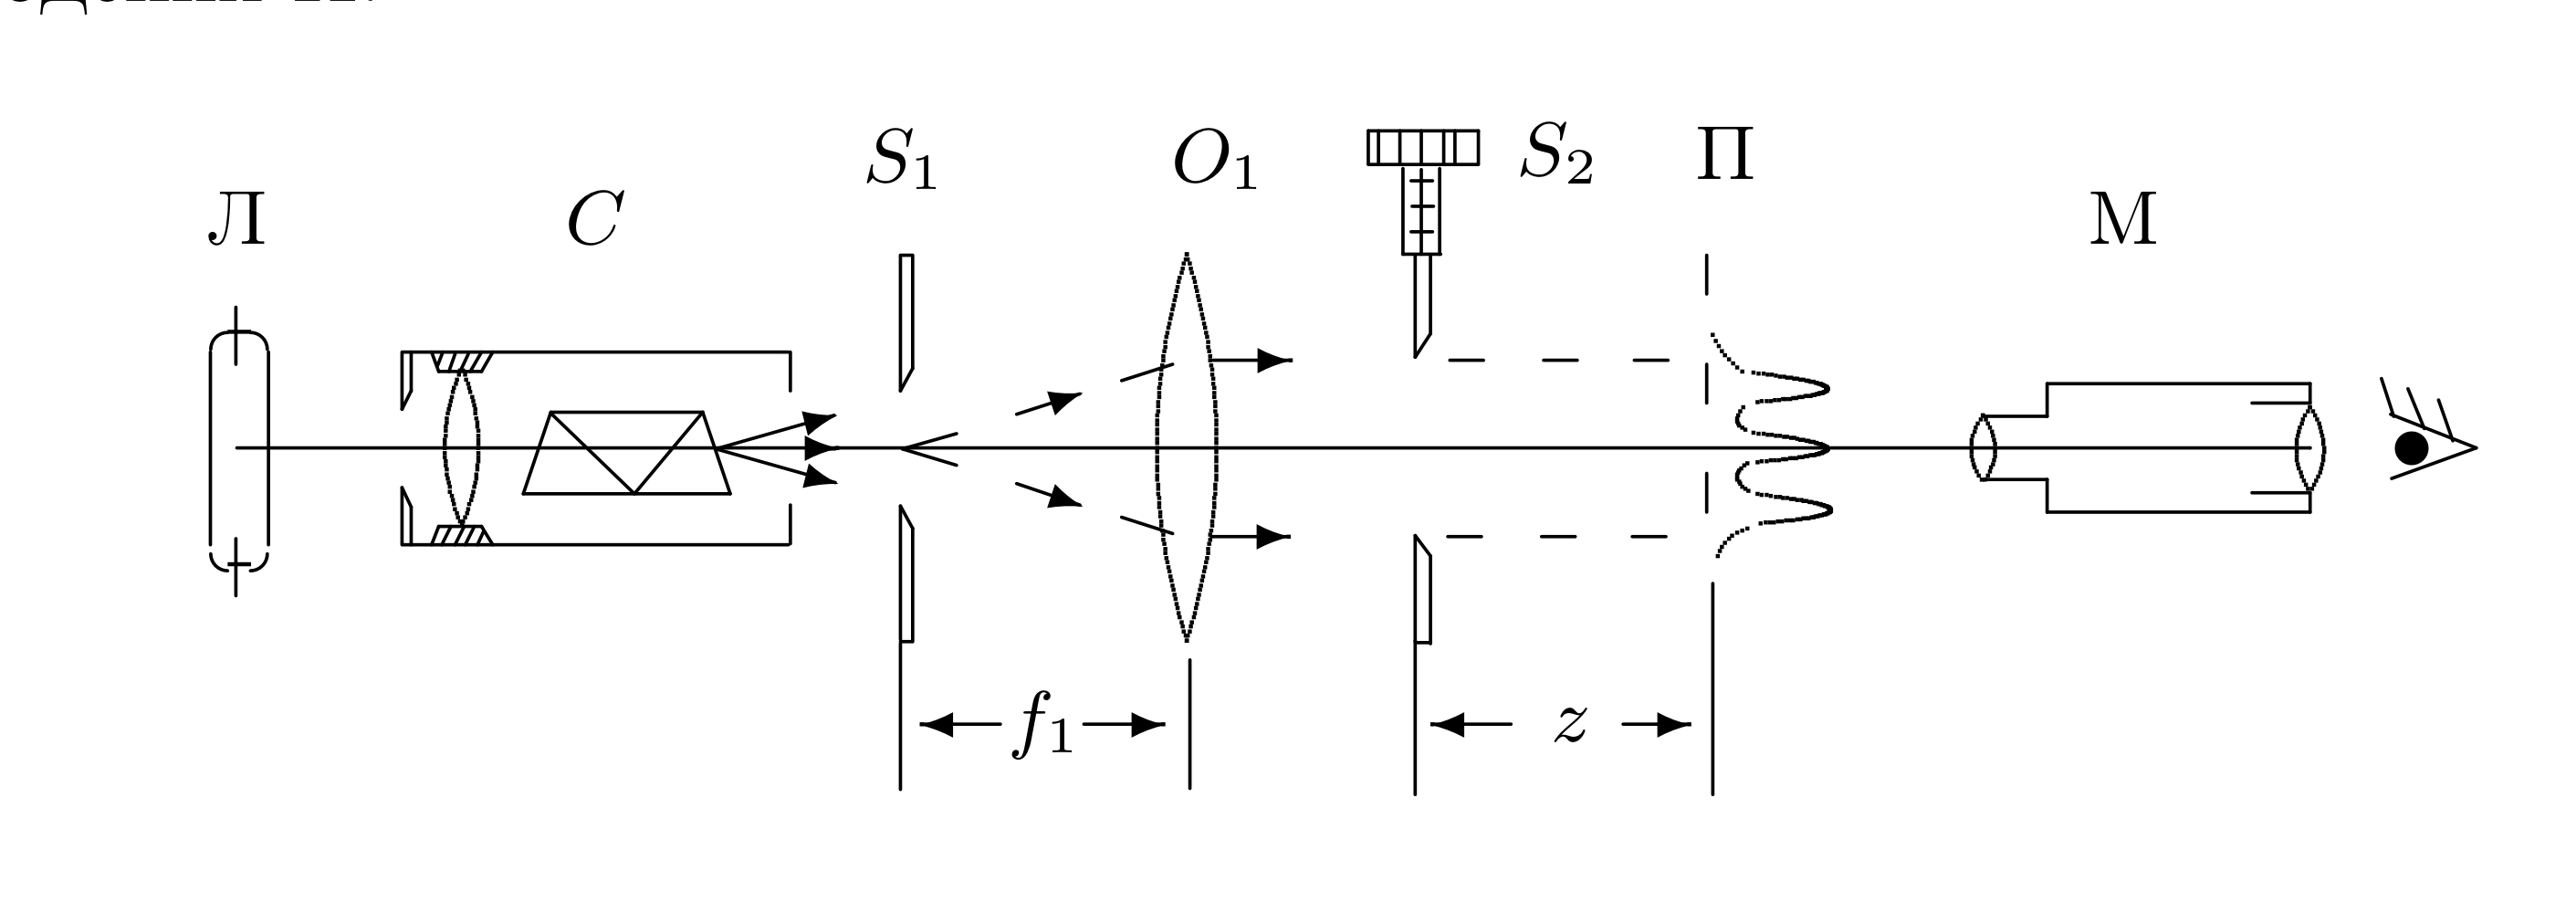
\includegraphics[scale=0.15]{4.3.1/alab.jpeg}
	\caption{Схема установки для наблюдения дифракции Френеля}
	\label{labA}
\end{figure}

Щель $ S_2 $ освещается параллельным пучком монохроматического света с помощью коллиматора, образованного объективом $ O_1 $, и щелью $S_1$, находящейся в его фокусе. На щель $ S_1 $ сфокусировано изображение спектральной линии, выделенной из спектра ртутной лампы Л при помощи простого монохроматора C, в котором используется призма прямого зрения. Распределение интенсивности света в плоскости наблюдения П проще всего рассчитывать с помощью зон Френеля (для щели их иногда называют зонами Шустера). При освещении щели $ S_2 $ параллельным пучком лучей (плоская волна) зоны Френеля представляют собой полоски, параллельные краям щели (рис. \ref{zone}). Результирующая амплитуда в точке наблюдения определяется суперпозицией колебаний от тех зон Френеля, которые не перекрыты створками щели. Графическое определение результирующей амплитуды производится с помощью векторной диаграммы --- спирали Корню. Суммарная ширина $ n $ зон Френеля (Шустера) определяется соотношением:

\begin{equation}\label{xin}
\xi_n = \sqrt{zn\lambda}
\end{equation}
где $ z $ --- расстояние от щели до плоскости наблюдения (рис. \ref{labA}), а $ \lambda $ --- длина волны.

\begin{figure}[H]
	\begin{center}
		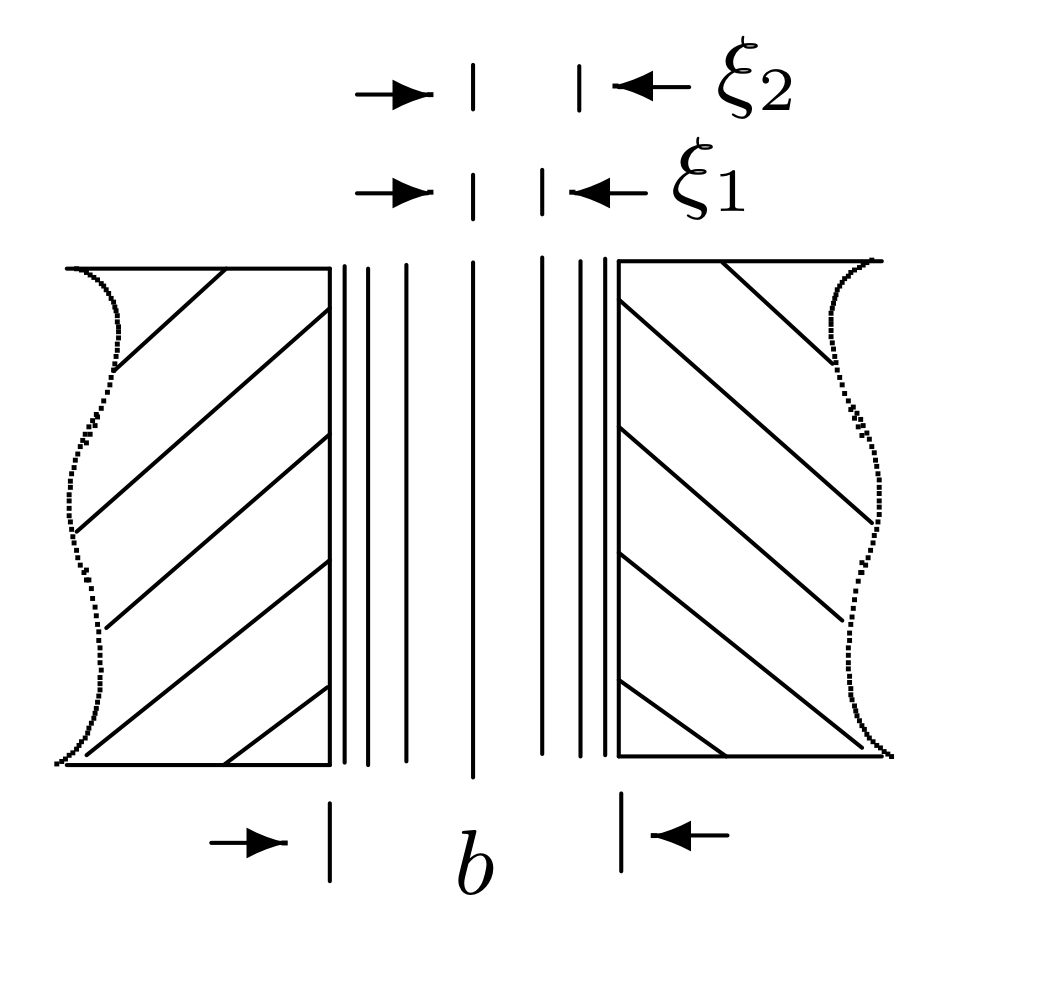
\includegraphics[scale=0.15]{4.3.1/zone.jpeg}
	\end{center}
	\caption{Зоны Френеля}
	\label{zone}
\end{figure}

Вид наблюдаемой дифракционной картины
на щели шириной $ b $ определяется волновым параметром $ p $ или числом Френеля $ C $ (число открытых полных зон):


\begin{equation}\label{}
p = \dfrac{\sqrt{z \lambda}}{b}, \qquad C = \dfrac{1}{p^2}
\end{equation}

\subsection{Дифракция Фраунгофера на одной щели}

На значительном удалении от щели, когда выполнено условие $ C \ll 1 $
(то есть ширина щели становится значительно меньше ширины первой
зоны Френеля, $ b \ll \sqrt{\lambda z} $), изображение щели размывается и возникает
дифракционная картина, называемая дифракцией Фраунгофера.

Дифракцию Френеля и Фраунгофера можно наблюдать на одной
и той же установке (рис. \ref{labA}). Однако при обычных размерах установки дифракция Фраунгофера возникает только при очень узких щелях.

\begin{figure}[H]
	\centering
	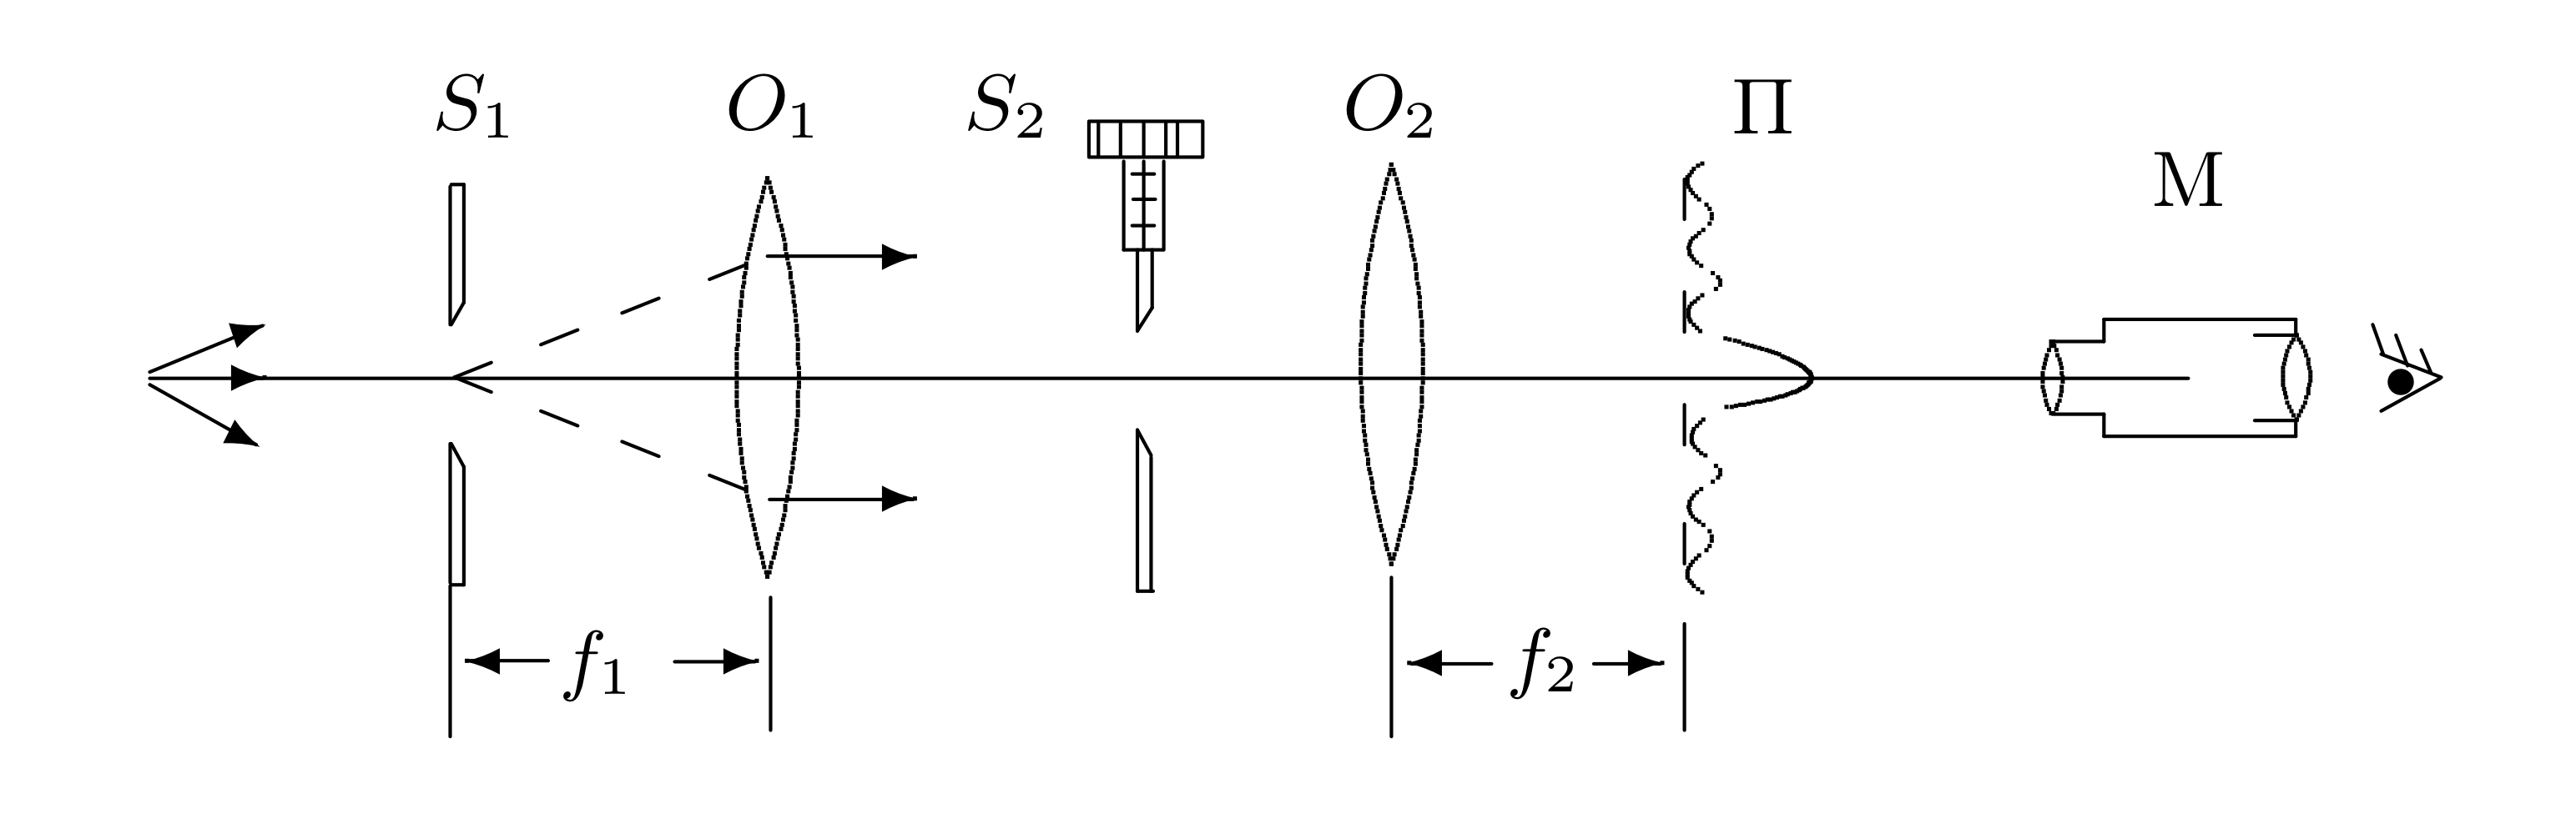
\includegraphics[scale=0.15]{4.3.1/blab.jpeg}
	\caption{Схема установки для наблюдения дифракции Фраунгофера на щели}
	\label{labB}
\end{figure}

Например, при $ z \approx  20-40 $  см и $  \lambda \approx 5 \cdot 10^{-5}  $   см получаем $  b \ll 0,3 $ мм. Поскольку работать с такими тонкими щелями неудобно, для наблюдения дифракции Фраунгофера к схеме, изображённой на рис. \ref{labA}, добавляется объектив $ O_2  $ (рис. \ref{labB}).

Дифракционная картина наблюдается здесь в фокальной плоскости
объектива $ O_2 $. Каждому значению угла $ \theta $ соответствует в этой плоскости точка, отстоящая от оптической оси на расстоянии

\begin{equation}\label{x}
x = f_2 \tg \theta \approx f_2 \theta
\end{equation}


плоскости наблюдается неискаженная дифракционная картина Фраунгофера. Эта картина соответствует бесконечно удалённой плоскости
наблюдения.

В центре поля зрения наблюдается дифракционный максимум (светлая полоса). При малых углах $ \theta $ положение минимумов (тёмных полос)
определяется, соотношением

\begin{equation}\label{theta_m}
\theta_m = m \dfrac{\lambda}{b}
\end{equation}

Расстояние $ x_m $ от тёмной полосы до оптической оси объектива $ O_2 $ пропорционально фокусному расстоянию $ f_2 $. Из \eqref{x} и \eqref{theta_m} следует 

\begin{equation}\label{xm}
x_m = m \dfrac{\lambda}{b} f_2
\end{equation}

Видно, что при малых углах минимумы эквидистантны, а расстояния $ \delta x $ между минимумами обратно пропорциональны ширине $ b $ щели $ S_2 $.



\subsection{Дифракция Фраунгофера на двух щелях}

Для наблюдения дифракции Фраунгофера на двух щелях в установке (рис. \ref{labB}) следует заменить щель $ S_2 $ экраном Э с двумя щелями
(рис. \ref{labC}). При этом для оценки влияния ширины входной щели на чёткость дифракционной картины вместо входной щели $ S_1 $ следует поставить щель с микрометрическим винтом. Два дифракционных изображения входной щели, одно из которых образовано лучами, прошедшими через левую, а другое --- через правую щели, накладываются друг на друга.

\begin{figure}[H]
	\centering
	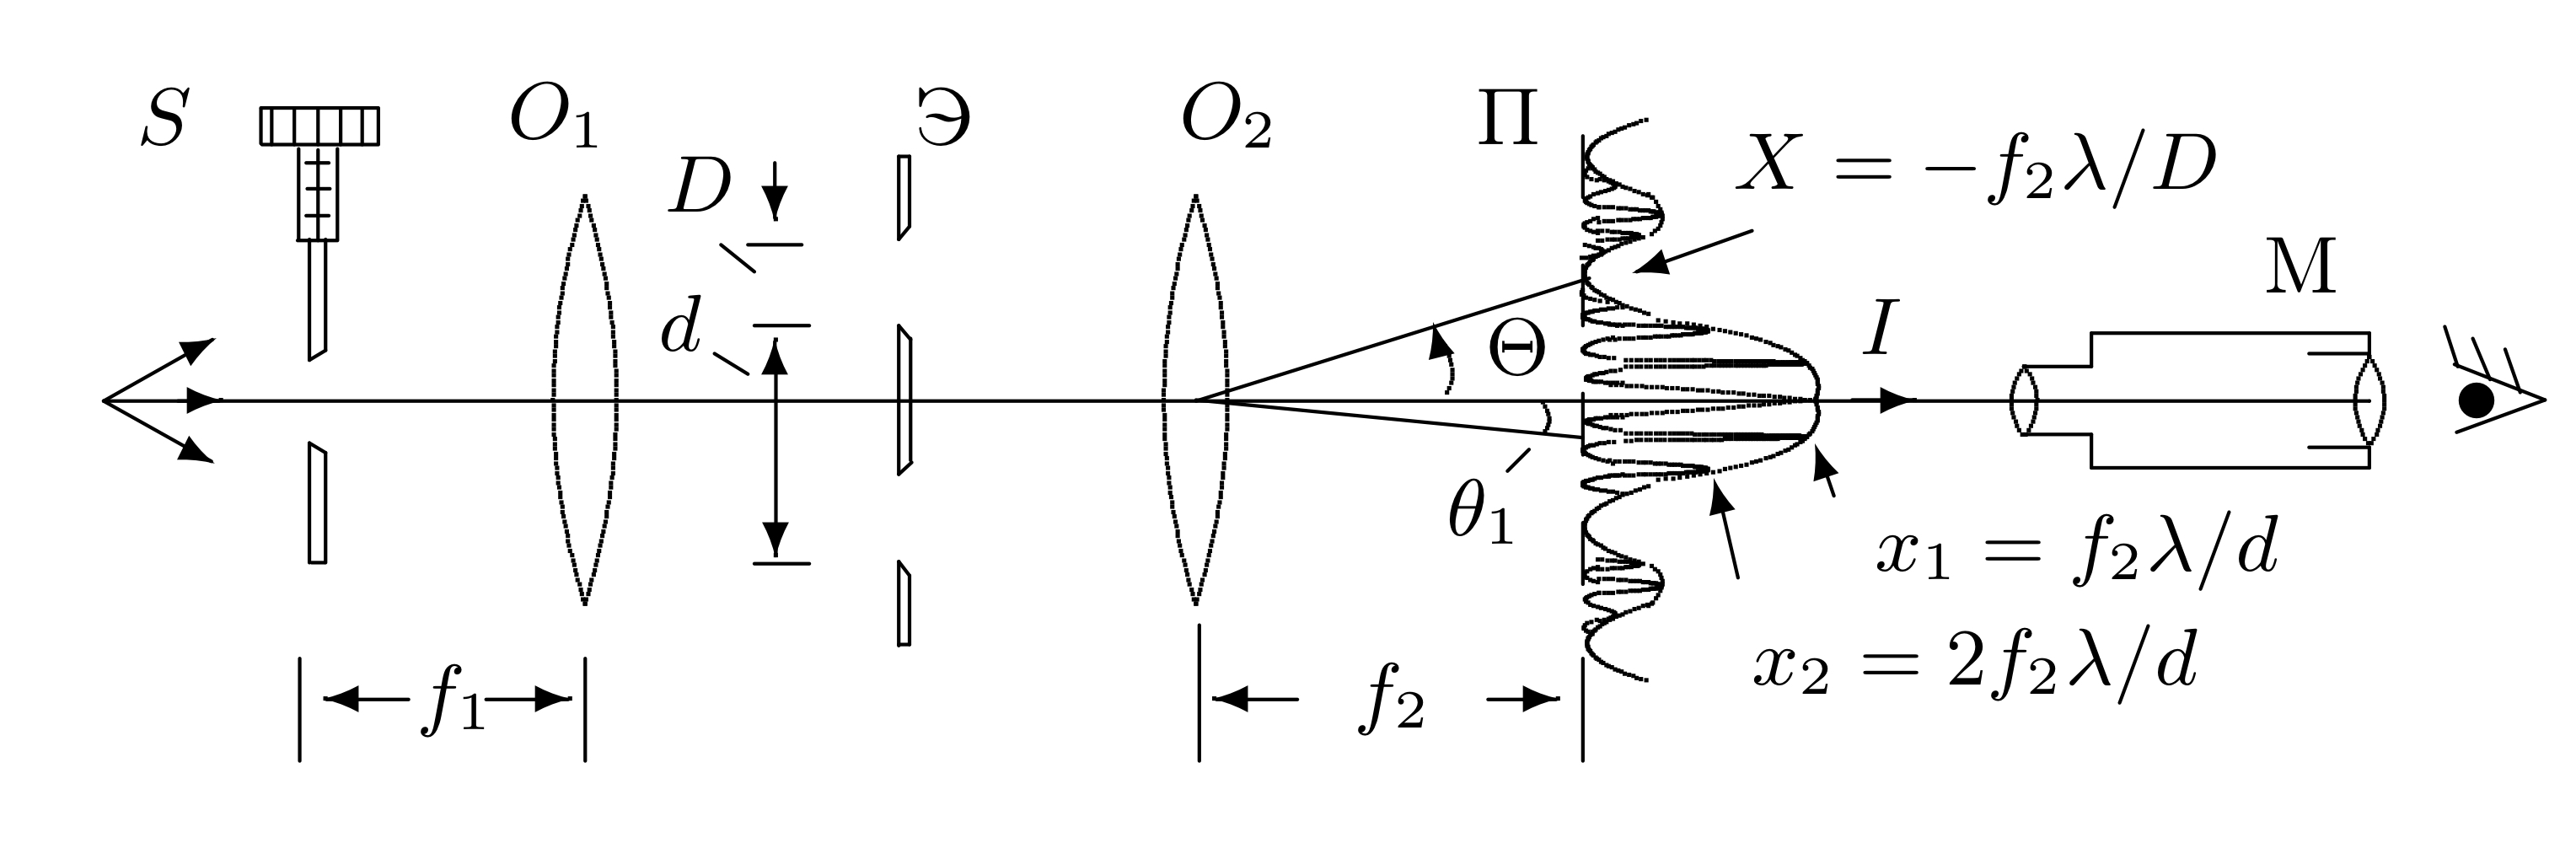
\includegraphics[scale=0.15]{4.3.1/clab.jpeg}
	\caption{Схема установки для наблюдения дифракции Фраунгофера на двух щелях}
	\label{labC}
\end{figure}

Если входная щель достаточно узка, то дифракционная картина
в плоскости П (рис. \ref{labC}) подобна той, что получалась при дифракции
на одной щели (рис. \ref{labB}), однако теперь вся картина испещрена рядом
дополнительных узких полос.
Угловая координата $ \theta_m $ интерференционного максимума $ m $-го порядка определяется соотношением

\begin{equation}\label{}
\theta_m = m \dfrac{\lambda}{b}
\end{equation}

где $ d $ --- расстояние между щелями. Линейное расстояние $ \delta x $ между соседними интерференционными полосами в плоскости П равно, поэтому

\begin{equation}\label{dx}
\delta x = f_2 \dfrac{\lambda}{d}
\end{equation}

На рис. \ref{labC} показано распределение интенсивности в фокальной плоскости объектива $ O_2 $. Штриховой линией (в увеличенном масштабе)
изображено распределение интенсивности при дифракции света на одиночной щели. Нетрудно оценить число n интерференционных полос,
укладывающихся в области центрального дифракционного максимума.
Согласно \eqref{xm} полная ширина главного максимума равна $ 2 f_2 \lambda /b $, где $ b $ ширина щели, отсюда

\begin{equation}\label{n}
n = \dfrac{2f_2 \lambda}{b} \dfrac{1}{\delta x} = \dfrac{2d}{b}
\end{equation}

При дифракции света на двух щелях чёткая система интерференционных полос наблюдается только при достаточно узкой ширине входной щели $ S $, которую можно рассматривать как протяжённый источник света размером $ b $. Для наблюдения интерференции необходимо, чтобы расстояние $ d $между щелями не превышало радиуса когерентности

\begin{equation}\label{}
d \ll \dfrac{\lambda}{b} f_1
\end{equation}

Здесь $ b $ --- ширина входной щели $ S $ и, следовательно, $  b/f_1 $ --- её угловая ширина. Таким образом, по размытию интерференционной картины можно оценить размер источника. Этот метод используется в звёздном интерферометре при измерении угловых размеров звёзд.

\subsection{Влияние дифракции на разрешающую способность оптического инструмента}

Установка, представленная на рис. \ref{labB}, позволяет исследовать влияние дифракции на разрешающую способность оптических инструментов.

Как уже было выяснено, линзы $O_1$ и $ O_2$ в отсутствие щели $S_2$ создают в плоскости П изображение щели $S_1$, и это изображение рассматривается в микроскоп М. Таким образом, нашу установку можно рассматривать как оптический инструмент, предназначенный для получения изображения предмета. При этом коллиматор (щель $S_1$ и объектив $O_1$) является моделью далёкого предмета, а объектив $O_2$ и микроскоп М составляют зрительную трубу, наведённую на этот предмет.
Щель $S_2$, установленная непосредственно перед объективом $O_2$, позволяет изменять эффективный размер объектива и, следовательно, разрешающую способность оптической системы.

\begin{figure}[H]
	\centering
	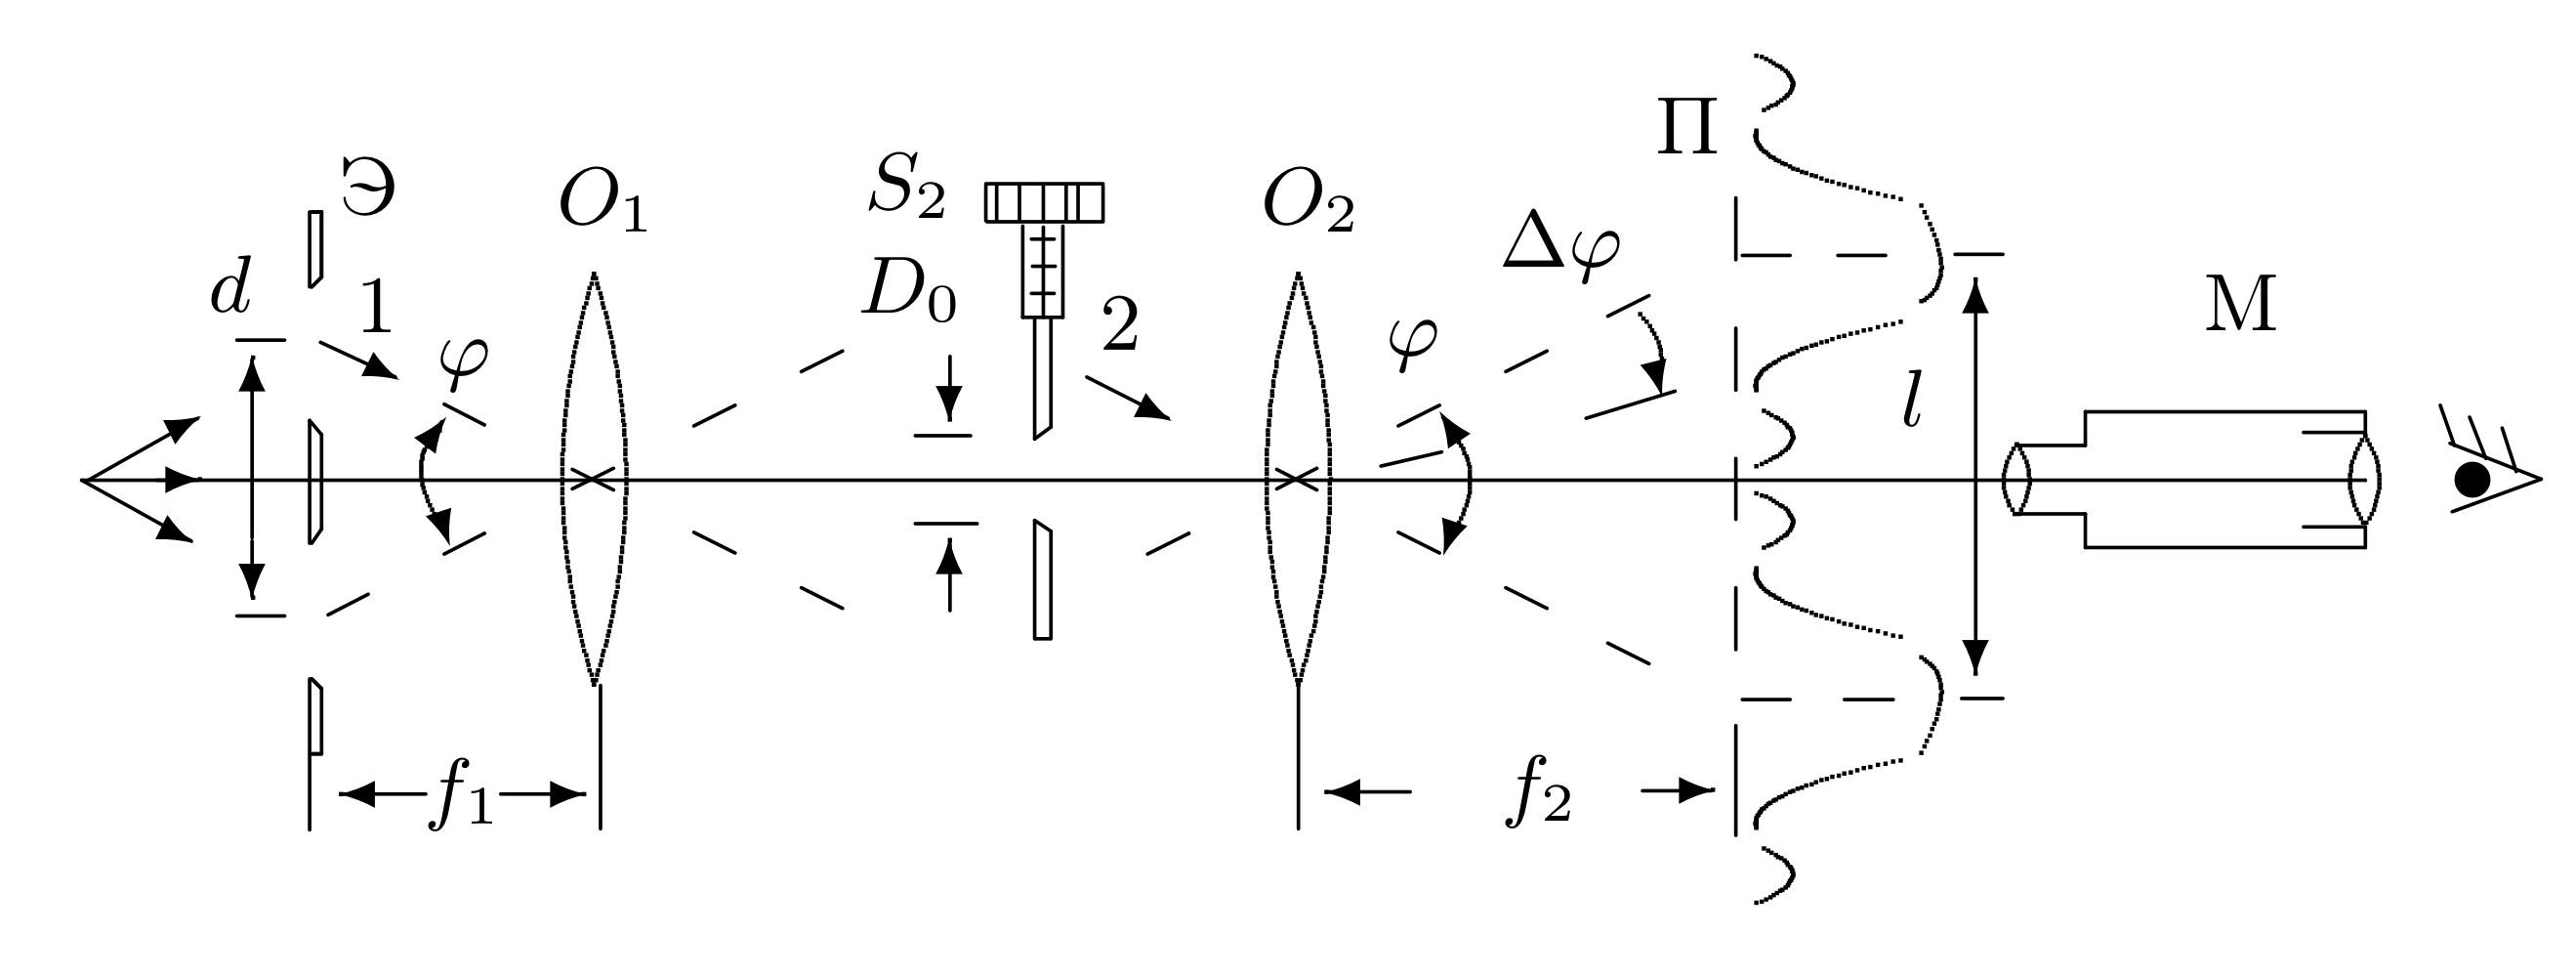
\includegraphics[scale=0.15]{4.3.1/dlab.jpeg}
	\caption{Схема установки для исследования разрешающей
		способности оптического инструмента}
	\label{labG}
\end{figure}

Поместим вместо щели $S_1$ экран Э с двумя узкими щелями, расстояние между которыми равно $d$ (рис. \ref{labG}). Тогда расстояние $l$ между изображениями щелей в плоскости П равно
\begin{equation}
l = \varphi f_2 = d \dfrac{f_2}{f_1},
\end{equation}
а ширина каждого изображения
\begin{equation}
\delta x \approx \dfrac{\lambda}{b} f_2
\end{equation}
определяется дифракцией света на щели $S_2$. Когда полуширина дифракционного изображения превышает расстояние между изображениями, то по виду дифракционной картины трудно определить, представляет собой источник двойную или одиночную щель.

Условия, при которых ещё можно различить, имеем мы дело с одной или двумя щелями, для разных наблюдателей различны. Для того чтобы исключить связанный с этим произвол, пользуются обычно критерием Рэлея, который приблизительно соответствует возможностям визуального наблюдения: изображения считаются различимыми, когда максимум одного дифракционного пятна совпадает с минимумом другого, а в условиях нашей задачи --- когда полуширина дифракционного изображения $\delta x$ совпадает с расстоянием $l$ между изображениями отдельных щелей:
\begin{equation}
\delta x \sim l \to \dfrac{\lambda}{b} \sim \dfrac{d}{f_1}.
\end{equation}

\section{Измерения, Обработка}

\subsection{Дифракция Френеля на щели}

Настроим установку согласно описанию. Не забудем проверить центрированность системы, чтобы избежать больших отклонений от параксиального приближения.

Определим нулевое положение микрометра. $m_0 = 0.373$ мм. Выставим ширину щели $b = 0.300 \pm 0.002$ мм. Найдем положение микроскопа, в котором видна одна дифракционная полоса в щели, а затем начнем приближать его, занося полученные измерения в таблицу.

\begin{equation}
	\xi_n = \sqrt{z_n n \lambda}
\end{equation}

Рассчитаем по полученным расстояниям радиусы i-х зон Френеля

\begin{center}
\begin{tabular}{|c|c|c|}
\hline 
n & z, см & $\xi_i$, мм \\
\hline
1&	2,95&	$0,254\pm	0,009$ \\
2&	1,85&	$0,284\pm	0,015$ \\
3&	1,35&	$0,297\pm	0,022$ \\
4&	1,05&	$0,303\pm	0,029$ \\
5&	0,9	&	$0,314\pm	0,035$ \\
6&	0,7	&	$0,303\pm	0,043$ \\
7&	0,62&	$0,308\pm	0,050$ \\
\hline
\end{tabular}
\end{center}

Для корректного рассчета усредненного значения ширины щели построим зависимость $z_n = \frac{\xi_n^2}{n \lambda}$. Абсолютные погрешности $z_n$ одинаковы и равны 2 мм.

\begin{figure}[H]
	\centering
	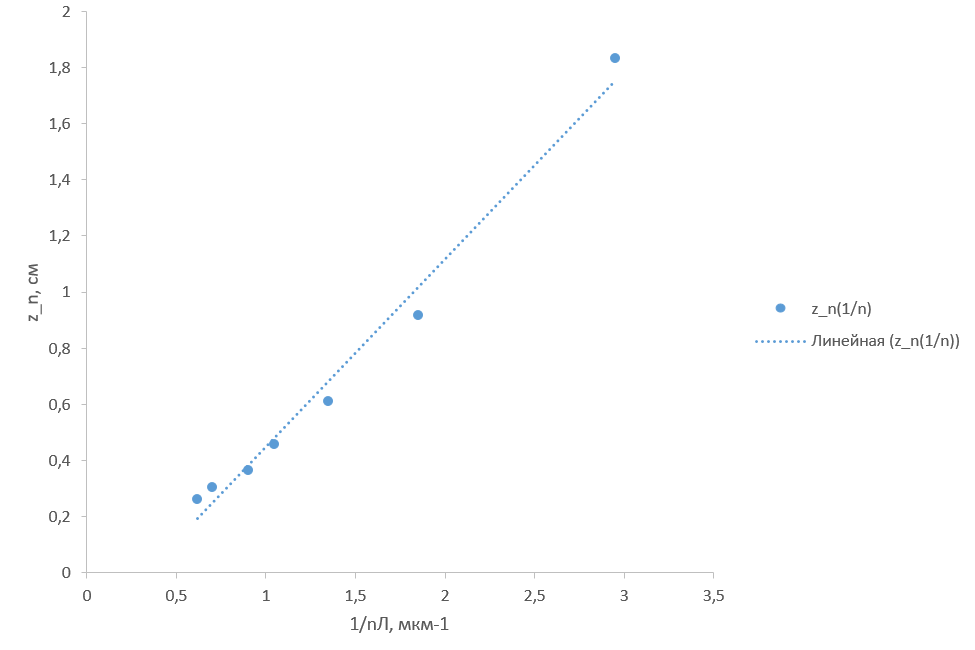
\includegraphics[scale=0.45]{gr1.png}
	\caption{Зависимость $z_n(\frac{1}{n \lambda})$}
	\label{labG}
\end{figure}





Найдем угловые коэффициенты прямых для каждой установки по МНК.

\[
	a = \frac{<x_i y_i> - < x > < y_i >}{< x_i^2> - < x_i >^2}
\]

\[
	b = < \nu_i > - a < N_i >
\]

Также рассчитаем их погрешности

\begin{equation}
	S_a^2 = \frac{< x_i^2>}{< x_i^2 > - < x_i >^2} \cdot \frac{<  b_i - b > ^2}{n - 2}
\end{equation}

Получим зависимость

\begin{equation}
	y = (0.00349 \pm 0.00072) + (1.469 \pm 0.085) \cdot 10^{-8} \cdot x
\end{equation}

Получим $\xi^2 = (1.469 \pm 0.085) \cdot 10^{-8}$ м$^2$

Тогда $b = \xi = 0.303 \pm 0.009$ мм.

Согласно показаниям шкалы на микроскопе $b = 0.34 \pm 0.04$ мм.

Итак, $b_\text{микрометр} = 0.300 \pm 0.002$ мм

$b_\text{френель} = 0.303 \pm 0.009$ мм

$b_\text{шкала} = 0.34 \pm 0.04$ мм

Все значения сходятся в пределах погрешности.

11) При неподвижном микроскопе и сжатии щели дифракционная картина сжимается и число полос уменьшается

14) Приведу результаты моделирования и наблюдений

В теории

\begin{figure}[!h]
	\centering
	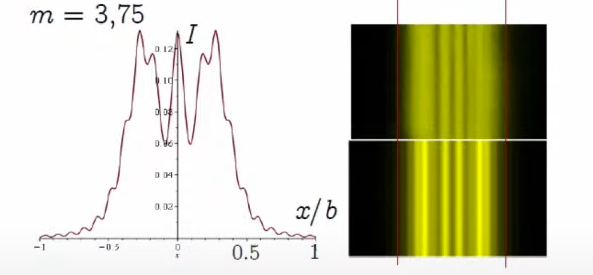
\includegraphics[width=1\textwidth]{th_fren.png}
	\label{fig:boiler}
\end{figure}

И на практике

\begin{figure}[!h]
	\centering
	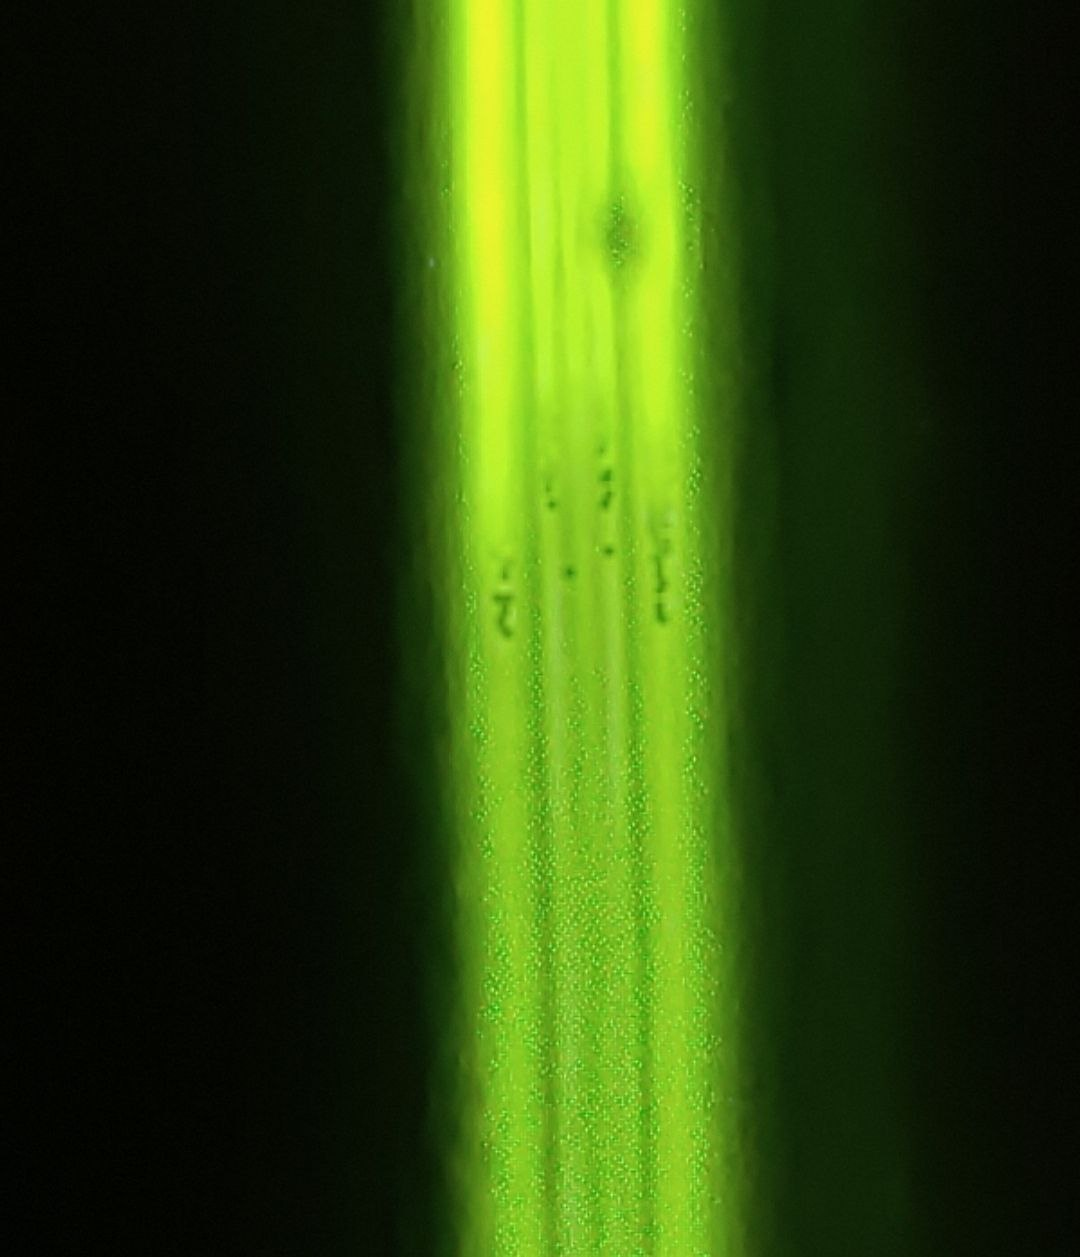
\includegraphics[width=0.5\textwidth]{pr_fren.jpg}
	\label{fig:boiler}
\end{figure}

Качественно картины похожы, хоть число открытых зон Френеля отличается.

\subsection{Дифракция Фраунгофера на щели}

Соберем установку. Зафиксируем ширину щели $b = 0.168$ мм по показаниям микрометра.

Фокусные расстояния линз $F_1 = 15.5$ см, $F_2 = 10.0$ см.

.

\begin{table}[H]
	\caption{Зависимость минимумов от их номера $ m $}
	\begin{center}
		\begin{tabular}{|c|c|c|c|c|c|c|c|} \hline
			$m$ & -3 & -2 & -1 & 0 & 1 & 2 & 3\\ \hline
			$ x_m $, мм  & 0.1 & 0.5 & 0.9 & 1.5 & 2.1 & 2.4 & 2.9 \\ \hline
		\end{tabular}
	\end{center}
	\label{tab2}
\end{table}

7) Погрешность определения координат оценю в 0.1 мм вследствие нечеткости максимумов и их тусклости(что все равно соотвествует полученной случайной погрешности)

Построю график зависимости координаты минимума от его порядка

\newpage

\begin{center}
	\Large $x(m)$
\end{center}

\begin{figure}[!h]
	\centering
	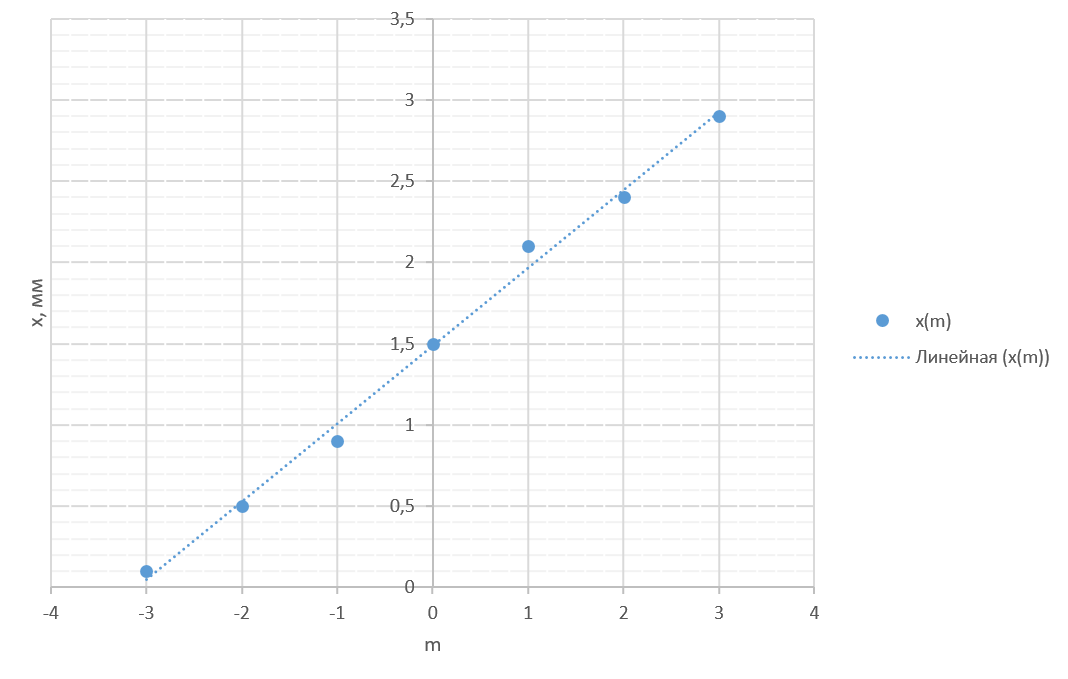
\includegraphics[width=1\textwidth]{fraun_pl.png}
	\label{fig:boiler}
\end{figure}

Из аппроксимации МНК и теории

\begin{equation}
	x_m = x_0 + m \frac{\lambda}{b} f_2 = (1.486 \pm 0.032) + (0.479 \pm 0.016) \cdot x
\end{equation}

Выражая из коэффициента наклона, $b = 0.171 \pm 0.006$ мм, что сходится с показаниями микрометра.

5) Картина соотвествует бесконечно удаленной плоскости наблюдения, поэтому смещение щели на картину не влияет.

6) Масштаб картины изменяется обратно пропорционально диаметру щели в соответствии с теорией.

\subsection{Дифракция Фраунгофера на двух щелях}

Заменим центральную щель пластиной с вырезанными 2-мя параллельными щелями. Полученная дифракционная картина выглядит так

\begin{figure}[!h]
	\centering
	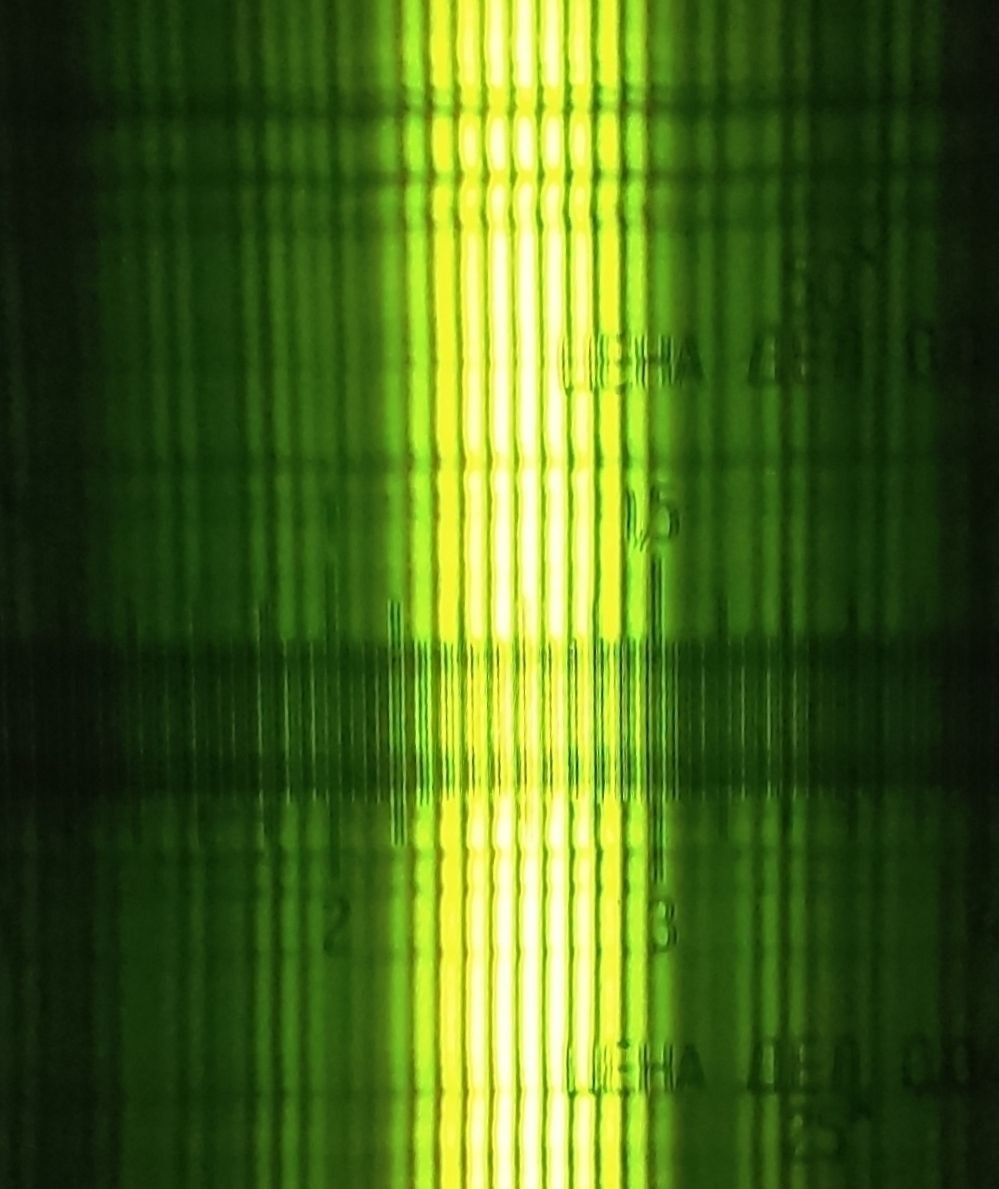
\includegraphics[width=0.5\textwidth]{2_fraun.jpg}
	\label{fig:boiler}
\end{figure}

\newpage

Ширина центрального максимума $x = 0.335 \pm 0.05$, соответствует 9 промежуткам, а всего полос $N = 10$. Тогда ширина одного промежутка $x_0 = 0.0372 \pm 0.006$ мм.

Тогда $d = \frac{f_2 \lambda}{\delta x} = 1.47 \pm 0.02$ мм

$b_0 = 0.12 \pm 0.01$ мм - показания микрометра, когда полосы исчезают. 

По формуле 10 из критерия Релея $b = \lambda \frac{f_1}{d} = 0.37 \pm 3$ мм. Тогда $n = \frac{2 d}{n} = 8 \pm 1$.

Прямые замеры по шкале микроскопа:

$d = 1.44 \pm 0.04$ мм
$b = 0.29 \pm 0.04$ мм

Полученные различными методами значения хорошо согласуются.

\subsection{Влияние дифракции на разрешающую способность оптического инструмента}

Изображения щелей начинают сливаться при ширине щели $b_0 = 0.13 \pm 0.1$ мм (показания микрометра).

Из критерия Релея $b_0 = \lambda \frac{f_1}{d} = 0.09 \pm 0.01$ мм

Довольно большое отклонение может быть вызвано субъективным завышением критерия Релея.

\section{Вывод}

При выполнении работы получились довольно однозназные и воспроизводимые результаты, что не может не подтверждать теорию.

\section{Ресурсы}

Расчет по МНК: метод-наименьших-квадратов.рф


\end{problem}
\end{document}